%%%%%%%%%%%%%%%%%%%%%%%%%%%%%%%%%%%%%%%%%
% Journal Article
% LaTeX Template
% Version 1.3 (9/9/13)
%
% This template has been downloaded from:
% http://www.LaTeXTemplates.com
%
% Original author:
% Frits Wenneker (http://www.howtotex.com)
%
% License:
% CC BY-NC-SA 3.0 (http://creativecommons.org/licenses/by-nc-sa/3.0/)
%
%%%%%%%%%%%%%%%%%%%%%%%%%%%%%%%%%%%%%%%%%
%----------------------------------------------------------------------------------------
%       PACKAGES AND OTHER DOCUMENT CONFIGURATIONS
%----------------------------------------------------------------------------------------
\documentclass[12pt, a4paper]{article}
\usepackage[english]{babel} % English language/hyphenation
\usepackage{amsmath,amsfonts,amsthm} % Math packages
\usepackage[utf8]{inputenc}
\usepackage{float}
\usepackage{wrapfig}
\usepackage{lipsum} % Package to generate dummy text throughout this template
\usepackage{blindtext}
\usepackage{graphicx} 
\usepackage{caption}
\usepackage{subcaption}
\usepackage[sc]{mathpazo} % Use the Palatino font
\usepackage[T1]{fontenc} % Use 8-bit encoding that has 256 glyphs
\linespread{1.05} % Line spacing - Palatino needs more space between lines
\usepackage{microtype} % Slightly tweak font spacing for aesthetics
\usepackage[hmarginratio=1:1,top=32mm,columnsep=20pt]{geometry} % Document margins
\usepackage[export]{adjustbox}
\usepackage{multicol} % Used for the two-column layout of the document
%\usepackage[hang, small,labelfont=bf,up,textfont=it,up]{caption} % Custom captions under/above floats in tables or figures
\usepackage{booktabs} % Horizontal rules in tables
\usepackage{float} % Required for tables and figures in the multi-column environment - they need to be placed in specific locations with the [H] (e.g. \begin{table}[H])
\usepackage{hyperref} % For hyperlinks in the PDF
\usepackage{lettrine} % The lettrine is the first enlarged letter at the beginning of the text
\usepackage{paralist} % Used for the compactitem environment which makes bullet points with less space between them
\usepackage{abstract} % Allows abstract customization
\renewcommand{\abstractnamefont}{\normalfont\bfseries} % Set the "Abstract" text to bold
\renewcommand{\abstracttextfont}{\normalfont\small\itshape} % Set the abstract itself to small italic text
\usepackage{titlesec} % Allows customization of titles
\usepackage{pagenote}
\makepagenote
\renewcommand\thesection{\Roman{section}} % Roman numerals for the sections
\renewcommand\thesubsection{\Roman{subsection}} % Roman numerals for subsections
\renewcommand\thesubsubsection{\Roman{subsubsection}} % Roman numerals for subsections 
\titleformat{\section}[block]{\large\scshape\centering}{\thesection.}{1em}{} % Change the look of the section titles
\titleformat{\subsection}[block]{\large}{\thesubsection.}{1em}{} % Change the look of the section titles
\titleformat{\subsubsection}[block]{\large}{\thesubsubsection.}{1em}{}

\newcommand{\horrule}[1]{\rule{\linewidth}{#1}} % Create horizontal rule command with 1 argument of height
\usepackage{fancyhdr} % Headers and footers
\pagestyle{fancy} % All pages have headers and footers
\fancyhead{} % Blank out the default header
\fancyfoot{} % Blank out the default footer

% \fancyhead[C]{Dept. of CSE, IIT Kanpur$\bullet$ Autumn 2016 $\bullet$} % Custom header text

\fancyfoot[RO,LE]{\thepage} % Custom footer text
%----------------------------------------------------------------------------------------
%       TITLE SECTION
%----------------------------------------------------------------------------------------
\title{
	\vspace{-34mm}
    \fontsize{24pt}{12pt}
    \selectfont\textbf{
    On segmentation of Nerve Structures \\ 
    in Ultrasound Images
    }
} % Article title

\author
{
    Manikanta Reddy D, \\
    Computer Science and Engineering, \\
    IIT Kanpur.\\
    \href{mailto:manikant@iitk.ac.in}{manikant@iitk.ac.in}
    \\
    \\
    Supervised by, \\ 
    Prof. Harish C. Karnick,\\
    Computer Science and Engineering, \\
    IIT Kanpur.\\
    \href{mailto:hk@cse.iitk.ac.in}{hk@cse.iitk.ac.in}
} % Author

\date{\Large Autumn, 2016}
%----------------------------------------------------------------------------------------

\begin{document}
\maketitle % Insert title
% \thispagestyle{fancy} % All pages have headers and footers
\begin{center}
\LARGE Overview
\end{center}
Pain is one of the most important aspects, that has to be properly managed, for easing the suffering of a patient and improve their quality of life. Pain management is typically done through the administration of narcotics, which also bring with them other unwanted effects. On the other hand introducing pain management catheters\footnote{\href{https://www.med.umich.edu/1libr/Anesthesiology/PeripheralNerveCatheterWhatIstIt.pdf}{Pain Management Catheters}}, that block or mitigate the pain at source, reduce dependency on the narcotics and speed up the recovery process. We will discuss the problem of identifying nerve structures in the region around neck so that the indwelling catheters are rightly placed and provide a pain free future. 

Accurately identifying the nerve structures, also called the \emph{Brachial Plexus}\footnote{\href{https://en.wikipedia.org/wiki/Brachial_plexus}{Wikipedia: Brachial Plexus}}, in the ultrasound images of the region around the neck can be modeled as an image segmentation problem. By placing the nerve structure in one class and the rest in the contrary, the problem is further simplified to a binary classification problem. Many methods exist to perform binary image segmentation, ranging from simple threshold based approaches to ones that use very deep neural networks. We will be discussing a method based on proposals by overlapping windows and the other, based on the U-net architecture\footnote{U-net: Convolutional networks for biomedical image segmentation\cite{ronneberger2015u}}. We will also look into how the choice of architecture of the neural net, makes the learning different in the deeper layers.  
\newpage
\tableofcontents
\newpage
\thispagestyle{fancy}
\section{Introduction}
The goal of any image segmentation algorithm is to represent the image in a more meaningful manner and to identify structures and boundaries around them. In its simplest form segmentation is assigning class labels to every pixel in the image. We'll be segmenting ultrasound images of a region around the neck.
\subsection{Problem}
The region of our interest is a collection of nerve structures called \emph{Brachial Plexus}, which extends over the spinal cord, through the neck and into the armpit. 
\begin{figure}[ht!]
\centering
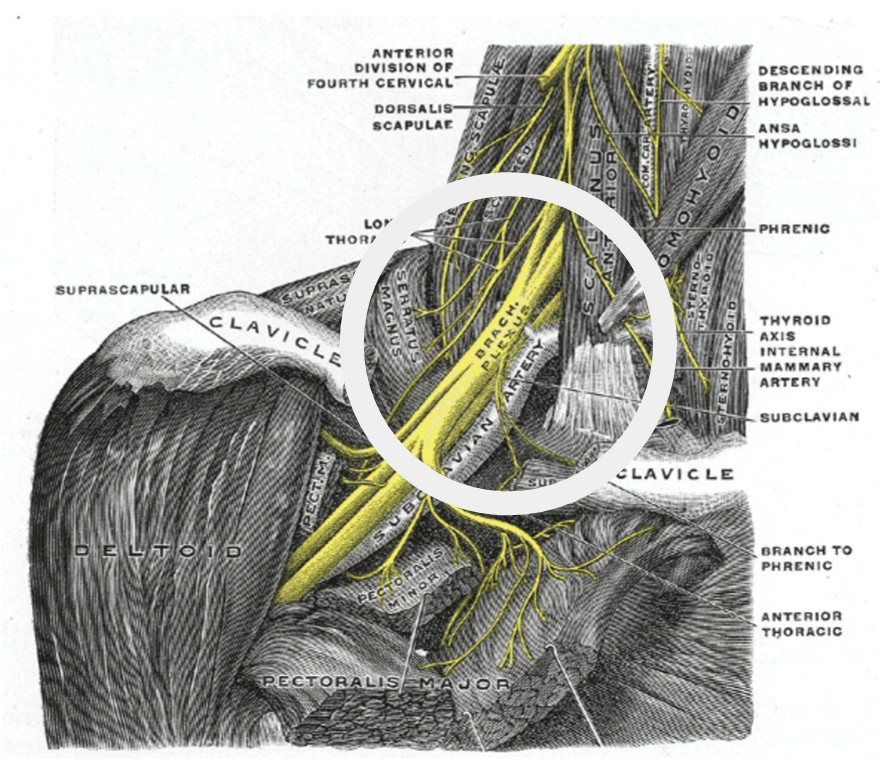
\includegraphics[width=120mm]{Brachial_Plexus.jpg}
\caption[The LOF caption]{Brachial Plexus\footnotemark}
\end{figure}
\footnotetext{Henry Vandyke Carter - Henry Gray (1918) Anatomy of the Human Body}
Identifying the accurate location of this nerve structure is a critical step in inserting the patients pain management catheter. The problem is posted as a challenge on \emph{Kaggle}\footnote{\href{https://www.kaggle.com/c/ultrasound-nerve-segmentation/}{Kaggle: Ultrasound Nerve Segmentation}} to build a model that can locate the plexus in a dataset of ultrasound images of the neck.
\section{Data}
The dataset provided consists of large training set of ultrasound images, in which the nerve structure is manually annotated by trained experts. The experts make their mark on the basis of their confidence of existence of BP in the image.

Given below are two images, one is the ultra sound image itself and the other is the human annotation.
\\
\begin{figure}[h] 
\begin{subfigure}{0.5\textwidth}
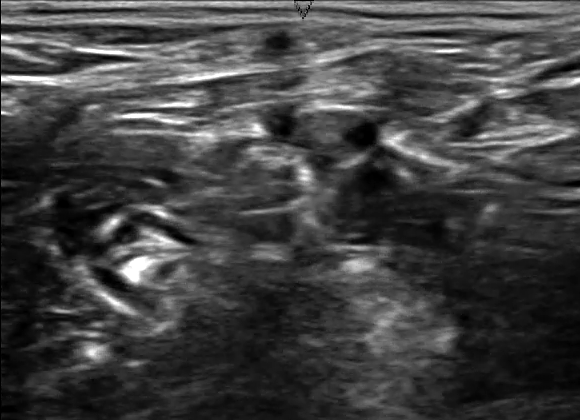
\includegraphics[width=\linewidth, height=5cm]{47_117.png} 
\caption{Ultrasound Image}
\label{fig:ultrasoundimage}
\end{subfigure}
\begin{subfigure}{0.5\textwidth}
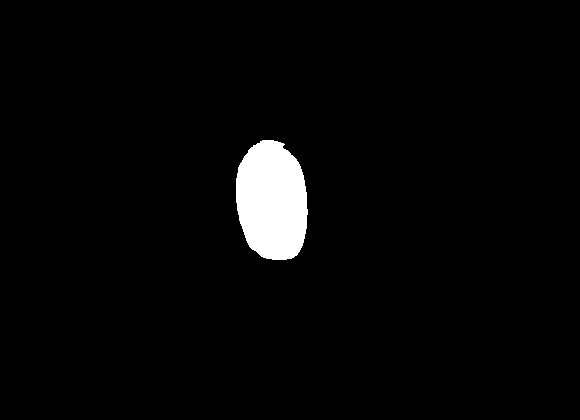
\includegraphics[width=\linewidth, height=5cm]{47_117_mask.png}
\caption{Human Annotation}
\label{fig:humanannotation}
\end{subfigure}
\caption{Sample Data from training set [Id : 47\_117]}
\label{fig:dataimage}
\end{figure}
The white region represents our region of interest. The model which we will build has to take the gray scale ultrasound image on the left as input and output a binary mask, similar to the binary image on the right. It has to be noted that the output is not gray scale. The intensities will be exclusively either 0 or 255.

\begin{figure}[h] 
  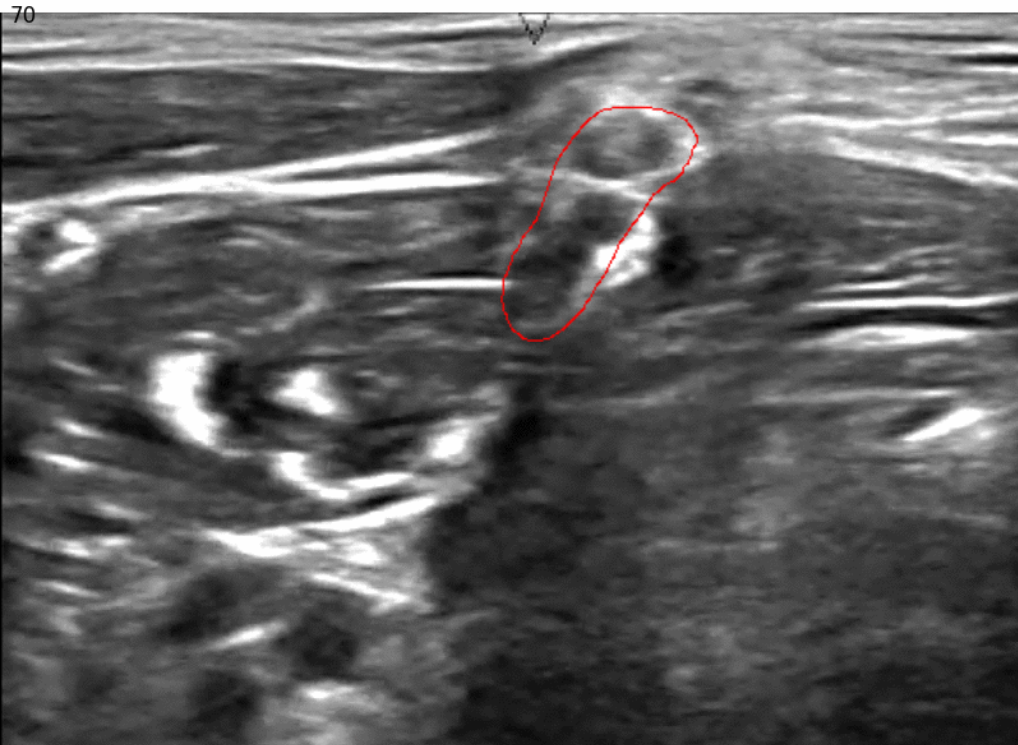
\includegraphics[width=\linewidth]{red_overlay.png}
  \caption{Image with overlay\\Notice the red boundary over the region of interest}
  \label{fig:overlayimage}
\end{figure}

Priori analysis of the data reveals that about 60\% of the images do not posses a mask, implying that they have no BP landmark. Hence we might not worry about the statistical bias in the supply of data. 

Other notable key points about the dataset,
\begin{itemize}
\item Image size: 580x420 pixels
\item 5635 training images
\item 5508 testing images
\item Noise and other artifacts present
\item Repetition of the images
\end{itemize}

\newpage
\subsection{Inconsistencies in the Data-set}
There are potential mistakes in the ground truth of the data. By this we mean that there are images, which are very similar to each other yet have differing masks\footnote{\href{https://www.kaggle.com/agalea91/ultrasound-nerve-segmentation/mislabeled-training-images/run/310043}{Mislabeled Training Images}}.

One of the images has a mask while the other doesn't and due to the nature of loss function we use for this problem, false positives and false negatives are penalized heavily.

The occurrence of such contrary images is highly likely in the test data-set provided. Coupled with the loss function, this particular empirical observation sets an upper bound on the results.

Another aspect of the image generation is the way they are produced. It seems that the images are frames of the ultrasound video feed, due to which we encounter multiple images which are actually the same frame.
\footnote{\href{https://www.kaggle.com/c/ultrasound-nerve-segmentation/data}{Data Description}}
\subsection{Dice Coefficient}
It has been suggested\footnotemark that \emph{Dice coefficient} be used as an error measure. Given two sets $A$ and $B$, dice index of them is, 
$$
Q =
\left\{
	\begin{array}{ll}
		 	\frac{|A\cap B|}{|A| + |B|} & \mbox{if } A\neq\phi | B\neq\phi \\
			1 & \mbox{otherwise}
	\end{array}
\right.
$$
This function penalizes any kind of wrong predictions. Just capturing the where and what is not enough, the prediction and truth have to be highly correlated. It is necessary that the binary outputs look as good as the real ones.
\footnotetext{\href{https://www.kaggle.com/c/ultrasound-nerve-segmentation/details/evaluation}{Evaluation}}


\section{Data Pre Processing}
In order to minimize the inherent inconsistencies, we pre process the whole of the data-set. 

\subsection{Image Down Scaling}
The images have been scaled down from 580x420 to 128x128. Other scales haven't been tested and could perform better. The reason to choose this scale is largely for programmatic ease and to avoid memory overflows in the system that's been used. \footnote{More experimentation has to be done, before any comment is made.}
\subsection{Removal of Inconsistent data}
In order to minimize contradictory data, we will remove all such pairs of images from data-set, which although are morphologically  similar posses different label masks. 

The closeness of two images was determined using cosine distance over block histograms of the images. Instead of dropping such images, propagating the masks over to the empty one, was also tried, but this didn't offer any convincing spike in the prediction power and rather degraded performance.
\subsection{Generating More Data}
One of the main advantages of working on medical images is that the objects of interest in the images are organic. They are indifferent to distortions and warping. Therefore we can freely transform the images by slightly changing them (Apply small affine transformations) to generate a completely different image that although different, can still be considered as a valid image for training. This compensates for the images we dropped previously.
\newpage
\section{Sliding Window Proposals}
This method is based on the idea that, the label a pixel will take depends on who its neighbors are and what labels they are taking. In order to encapsulate the information about what and how the neighbors of a pixel are doing, we consider a window around the pixel and map the pixels to a functional value and then use this functional value as a measure of confidence the window has, in the pixel, towards a particular class.
\begin{figure}[h] 
\begin{subfigure}{0.5\textwidth}
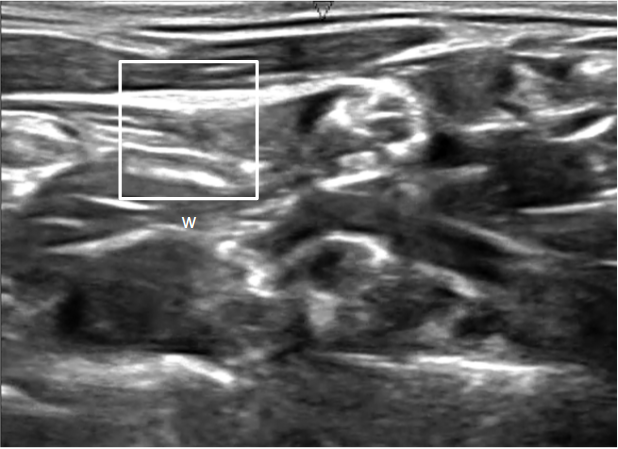
\includegraphics[width=\linewidth, height=5cm]{Selection_001.png} 
\caption{Ultrasound Image with window}
\label{fig:ultrasoundimagewithwindow}
\end{subfigure}
\begin{subfigure}{0.5\textwidth}
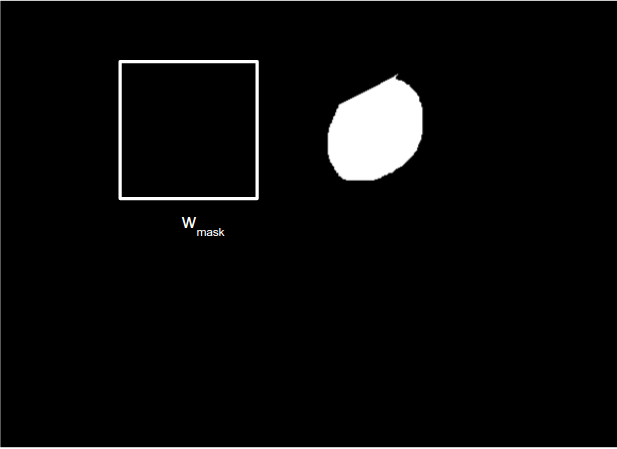
\includegraphics[width=\linewidth, height=5cm]{Selection_002.png}
\caption{Mask with corresponding window }
\label{fig:humanannotationwithwindow}
\end{subfigure}
\caption{Window Illustration [Id : 1\_85]}
\label{fig:dataimage2}
\end{figure}
\\
In the figures above, both the images have the window overlay, in white, at the same location. We call such windows \emph{corresponding} windows. They are capturing information from the same region, albeit in a different plane.
\subsection{Sliding Windows}
We'll consider $w$ as the window in the ultrasound image, or $x$, and $w_{mask}$ as the corresponding window in the mask image, or $y$. Every pixel in the image has some intensity value given by some intensity function $I:p_i \rightarrow (0,255)$. The window($w$) will contain some finite number of pixels and can be written as a set of all the pixels in the window as $$w = \{p_i / p_i \in w\}$$ or in a vector form as $$w = (I(p_1), I(p_2), ..., I(p_i), ...). \#\footnotemark$$
\footnotetext{We consider that, all windows are of same width and height, thus are of same dimension.}
Henceforth, $w_j$ will be the window in mask and ${w_{mask}}_j$ is the corresponding window in the mask and $W$ be range space of all windows. We can see that all windows over an image will therefore be unique sets of pixels. These sets may overlap, that is, a pixel can be present in multiple windows. 
\\
In our method, we try to build two functions $\Gamma: W\rightarrow [0,1]$ and $\Theta: W\rightarrow [0,1]$ such that 
$$\Gamma(w_j) = \Theta({w_{mask}}_j)$$

For our problem we define $\Theta$ as the mean of binary values of pixels in the window.
$$\Theta({w_{mask}}_j) = \frac{\sum\limits_{p_i \in {w_{mask}}_j}^n I(p_i)}{n} $$
We approximate $\Gamma$ as a logistic regression model and learn it through training which can be setup easily by dividing the images into sliding boxes with overlapping (some stride length). These boxes can be considered as windows. 
\\
$\Theta$ in a practical sense gives us an idea of how much interesting region it contains. $\Gamma$ then tries to figure out what feature of the original pixels generates such interesting region. $\Gamma(w)$ is the probability that the window has some mask.\\
By the end of this we land up with $\Gamma$, a function capable of predicting how much of the window belongs to the region of interest.
\subsection{The Proposals}
If we are able to somehow predict the class of a pixel our problem is done. We have already devised a way of relating the windows to region of interests. We now try to devise a way to use the information about windows for pixels. 

Every pixel in the image will belong to some finite number of windows, owing to the way how the windows are built. Every such window will capture some neighborhood of our pixel. Thus windows can be considered good representatives of the neighborhoods of the pixel. Any operation the window is an operation on the neighborhood. 

If a pixel neighborhood holds some property, it is very \emph{likely} that the property will hold for the pixel too. If windows have some probability of having some mask, so does the pixel. A window makes a proposal for a pixel to be a pixel in region of interest.

Since a pixel can belong to multiple windows, multiple neighborhoods have an affect on it simultaneously. We now make an important assumption that multiple neighborhoods affect the pixel \emph{independently}.

Thus using the above arguments, we define the probability$(P(p_i))$ that a pixel $p_i$ will be a pixel in region of interest as
$$ P(p_i) = \prod\limits_{p_i \in w_j} \Gamma(w_j) $$
Using this probability as a measure and by choosing appropriate thresholds, we can generate masks for any ultrasound image.
\newpage
\section{Neural Networks}
\subsection{Encoder-Decoder}
We are motivated by a simple desire to preserve spatial locality of the region of interest in the context of the entire image. We built a simple Encoder-Decoder network to do the same. 

We hope that the network learns a representation just enough to distinguish pixels of the nerve structure from the rest. 

\begin{figure}[h] 
  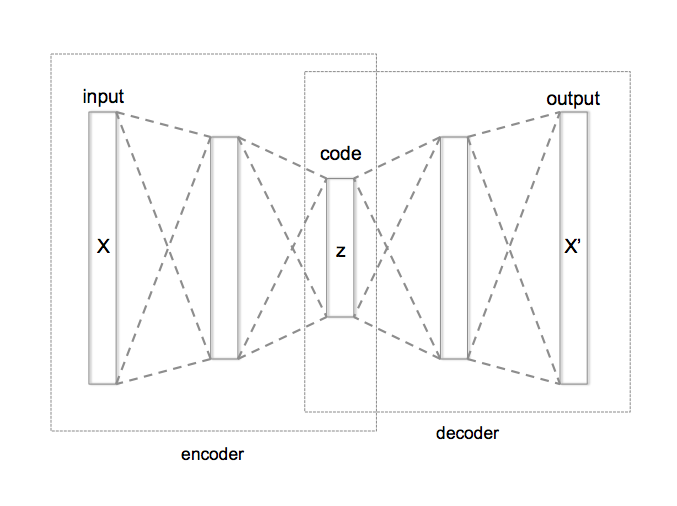
\includegraphics[width=\linewidth]{Autoencoder_structure.png}
  \caption[ ]{Encoder Decoder\footnotemark}
  \label{fig:autoencoder}
\end{figure}
\footnotetext{By Chervinskii - Own work, CC BY-SA 4.0, \href{https://commons.wikimedia.org/w/index.php?curid=45555552}{wikimedia}}

The network built was 4 pool layers deep with 3 convolutions in each layer. There is a simple contracting path and then a expanding path, that embed the information present in the entire image into lower dimensional vectors. The size of this vector is halved at every pool layer.

Autoencoders\cite{baldi2012autoencoders} can capture the context of the image in a very good manner in the representation it learns, but doesn't perform well when trying to learn the spatial localization present in the image.

In other words, this network captures the \emph{'what'} in the image but not the \emph{'where'} that particular answer to 'what' is present.
\newpage
\subsection{U-net}
We understand that the encoder decoder fails at one particular learning problem, capturing the spatial localization. In order to achieve this, all we have to do is provide the spatial information as well. 

We do so by combining the high resolution features from the contracting path with the up-sampling features in the expanding path. 

\begin{figure}[h] 
  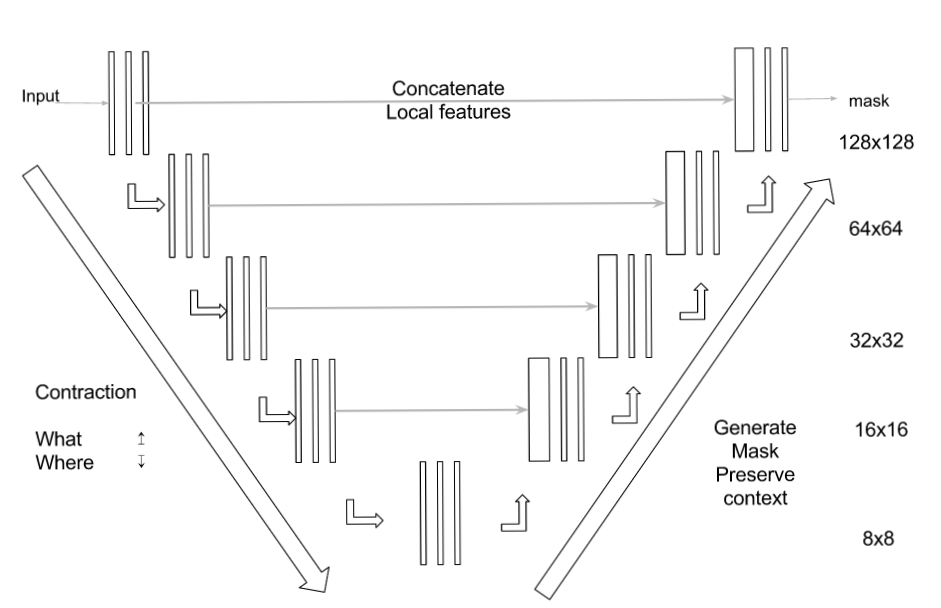
\includegraphics[width=\linewidth]{unet.png}
  \caption[ ]{U-net}
  \label{fig:unet}
\end{figure}

U-net\cite{ronneberger2015u} has two parts. i) Encoder and ii) Decoder. The first part is simple convolution network that embeds the image into lower dimensional vectors. The second part is also a simple upsampling network, but, with a change.

At every pooling step in the encoder network, we collect the vectors and feed them (concatenate with) the upsampled vectors from the previously layer in the decoder network. (Note the \emph{Concatenate local features} step in the image.

We are forcing the network to give emphasis on the high resolution features that are lost during the encoding step. During the contraction phase, the \emph{'what'} in the image is highly consolidated, \emph{'where'} is lost. The concatenation step, forces the network to relearn the \emph{'where'}, which it ignored in the contraction.

The final output will thus contain both the context and localization information in it. 
\subsection{Dreams}
Dreams\footnotetext{Inceptionism: Going deeper into neural networks\cite{mordvintsev2015inceptionism}} are a good way to visualize what the features, the filters are learning. They represent what kind of input ,\emph{excites}, the filters. 
\footnote{\href{https://blog.keras.io/category/demo.html}{Deep Dreams}}
\begin{figure}[h] 
\begin{subfigure}{0.5\textwidth}
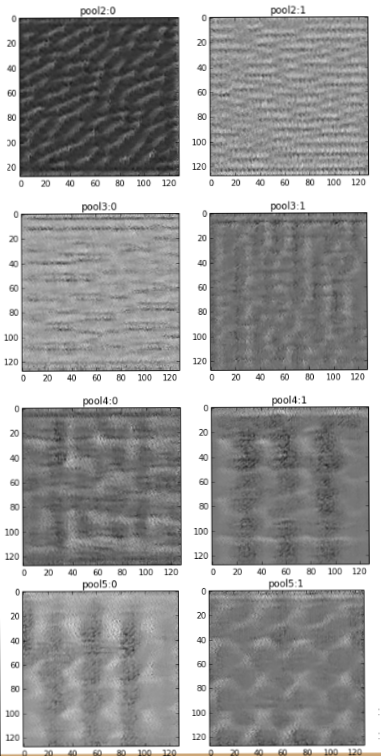
\includegraphics[width=\linewidth,height=15cm]{autoencoder_dream.png} 
\caption{Autoencoder's Dreams}
\label{fig:autoencodersdream}
\end{subfigure}
\begin{subfigure}{0.5\textwidth}
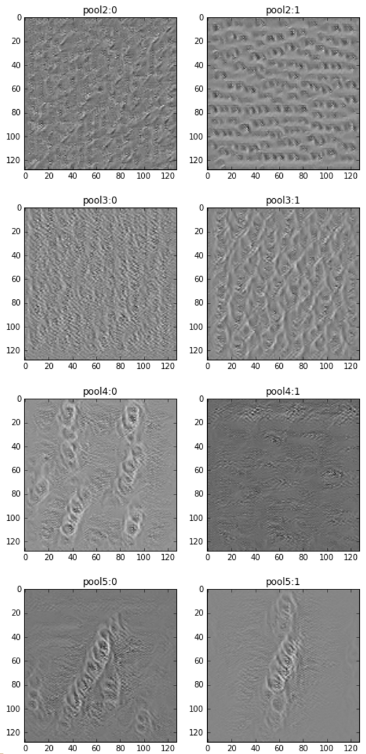
\includegraphics[width=\linewidth, height=15cm]{unet_dream.png}
\caption{Unet's Dream}
\label{fig:unetsdream}
\end{subfigure}
\caption{Dreams\\Notice the fibrous structures in U-net's dream}
\label{fig:dreams}
\end{figure}

As you can clearly see, U-net responds well to images with Brachial Plexus, something that autoencoder failed. Autoencoder would respond very well to ultrasound images of the neck, but can't find where exactly this nerve structure is present in it.
\section{Post Processing}
The output generated by any of the methods discussed is just a probability map of every pixel's likeliness to be in the region of interest. But as the problem demands in order to score, we should have output masks that would be as close to human like annotations. In order to convert this probability map into an annotation like image we employ different techniques.

\subsection{Thresholding}
We could simply set a threshold over the probability and generate binary outputs. But this solution, puts forward a serious problem.
\\
\begin{wrapfigure}{r}{0.5\textwidth}
\centering
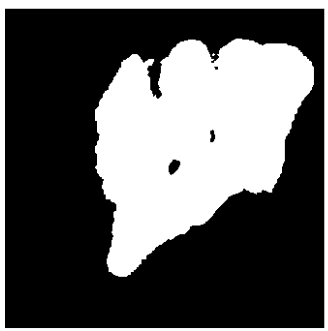
\includegraphics[width=0.48\textwidth, height=5cm]{holes.png} 
\caption{Discontinuity due to thresholds}
\label{fig:holeinthewall}
\end{wrapfigure}
On what basis do we chose the threshold? Certainly it is not the visual appeal. We should also not try to train a model to learn the threshold, because if something like that were possible, 
it would have been picked up by the model itself (at least in the neural networks).

The second problem is related to the discontinuous maps it can create. The threshold can be set in such a way that a certain region in the middle can be labeled the other way.
\\
The problem of undesired holes can be solved by applying a \emph{morphological} closing method, but still we would not have outputs that look human like.

\subsection{PCA based cleaning}
The desire to generate human-like annotations, points us to the question, what makes a mask human-like? Can we learn this too? We have many images that can teach us to generate such masks. 

In order to learn such features, we train a PCA model on all training masks, with region of interest. The PCA model will then give us some \emph{Eigen Masks}, or the inner features of drawing an annotation. Using a linear combination of these eigen masks, we should be in principle able to generate masks, that look like human annotated masks.
\begin{figure}[h] 
\begin{subfigure}{0.5\textwidth}
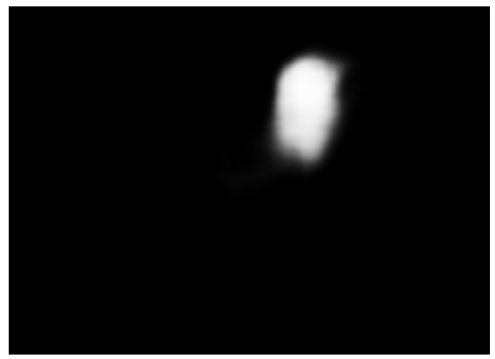
\includegraphics[width=\linewidth,height=5cm]{probability_mask.png} 
\caption{Probability Map}
\label{fig:probabilitymap}
\end{subfigure}
\begin{subfigure}{0.5\textwidth}
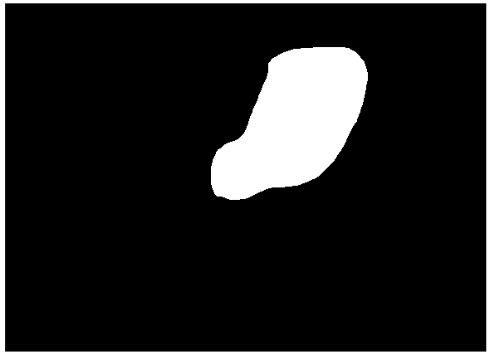
\includegraphics[width=\linewidth, height=5cm]{pca_cleaned.png}
\caption{PCA cleaned Mask}
\label{fig:pcamask}
\end{subfigure}
\caption{PCA transformation of probability masks}
\label{fig:pcatransform}
\end{figure}
\\
\section{ Results}
The results are computed by taking the mean of Dice score of the predicted masks with the annotated masks. The scores shown here are generated by kaggle.
\begin{table}[H]
\caption{Average Dice Coefficients}
\label{Tabel1}
\centering
\begin{tabular}{|l | c |}
\hline
Model & Best Dice Score \\
\hline
Blank submission & 0.53449	\\
Proposal Based &  0.56527\\
Autoencoder & 0.62322	\\
U-net (without PCA) & 0.66890 \\
U-net (with PCA) & 0.68719 \\
\hline
\end{tabular}
\end{table}
A blank submission, itself gives us a score of $0.53$ indicating that about half of the images do not contain any mask. 

The proposal based method used windows of size $30x30$ at a stride length of $10$. Experimentation with respect to window size and length is yet to be done.

The auto-encoder based method was a huge jump from previous solutions, as it was capable enough to capture the nerve structures as we have seen. 

Introducing extra connections in the encoder-decoder network to build the U-net brought the score up by $4\%$, indicating a strong learning of localization information. 

Post processing using PCA cleaning definitely brought a final bump in the score by about $2\%$. A much better post processing could also work.


% Bibilography
\renewcommand\refname{\vskip -1cm}
\section{References}
\bibliography{bib.bib}
\bibliographystyle{ieeetr}

\end{document}
